%                                                                 aa.dem
% AA vers. 9.1, LaTeX class for Astronomy & Astrophysics
% demonstration file
%                                                       (c) EDP Sciences
%-----------------------------------------------------------------------
%
% \documentclass[referee]{aa} % for a referee version
%\documentclass[onecolumn]{aa} % for a paper on 1 column  
%\documentclass[longauth]{aa} % for the long lists of affiliations 
%\documentclass[letter]{aa} % for the letters 
%\documentclass[bibyear]{aa} % if the references are not structured 
%                              according to the author-year natbib style

%

\documentclass{aa}  

%
\usepackage{graphicx}
\usepackage{amsmath,amsfonts,amssymb}
\usepackage{natbib}


%%%%%%%%%%%%%%%%%%%%%%%%%%%%%%%%%%%%%%%%
\usepackage{txfonts}
\usepackage{xcolor}

\usepackage{blindtext}
%%%%%%%%%%%%%%%%%%%%%%%%%%%%%%%%%%%%%%%%
% \usepackage[options]{hyperref}
% To add links in your PDF file, use the package "hyperref"
% with options according to your LaTeX or PDFLaTeX drivers.
\usepackage{float}
%\usepackage{stfloats}
\usepackage{dblfloatfix}
\usepackage{afterpage}
\usepackage{ifthen}
\usepackage[morefloats=12]{morefloats}

\usepackage{placeins}
\usepackage{multicol}
%\usepackage[breaklinks,colorlinks,citecolor=blue]{hyperref}
\bibpunct{(}{)}{;}{a}{}{,}
\usepackage[switch]{lineno}
\definecolor{linkcolor}{rgb}{0.6,0,0}
\definecolor{citecolor}{rgb}{0,0,0.75}
\definecolor{urlcolor}{rgb}{0.12,0.46,0.7}
\usepackage[breaklinks, colorlinks, urlcolor=urlcolor,
    linkcolor=linkcolor,citecolor=citecolor,pdfencoding=auto]{hyperref}
\hypersetup{linktocpage}
\usepackage{bold-extra}
\usepackage{lipsum}

%Planck style file, to be used with A&A style to produce Planck papers for publication.
%
% version 28 September 2010 --- useful macros --- CRL
% version 17 October 2010   --- first cut at important instrument values, from Daniele Mennella and
%                               Francois Bouchet, 13 October 2010 --- CRL
% version 18 October 2010   --- LFI FWHM changed to one value per feed, rather than M & S separately
%                               LFI FWHM uncertainties added for individual feeds.  Corrections made
%                               to LFI values. --- Andrea Zacchei
% version 24 October 2010   --- added to and corrected definitions.  No changes made to instrument
%                               quantities. --- CRL 
% version 31 October 2010   --- added definition of \muKHz. --- CRL
%
% version 15 November 2010  --- fixed conflict with aa.cls in definition of \endtable
%                               by naming the command below "\endPlancktable".  See section
%                               13.16 of the Style Guide.
%
% version 06 December 2010  --- Set up names with and without units.
%                               Add \allearlypapers command to ensure that all early papers are
%                               included in the reference list.
%                               Define macro for the name of the 4He JT cooler.
%
% version 07 December 2010  --- removed extraneous "planck2011-1.2" entry in \allearlypapers
%
% version 12 December 2010  --- added \endPlancktablewide command to set tablenotes to the full
%                               page width in the \begin{table*}...\end{table*} environment when
%                               the ``twocolumn'' option is specified in the \documentclass command.
%                               (It would be more elegant to extract the appropriate width from the
%                               aa.cls system at the time of execution, but that is buried more
%                               deeply in the system than I investigated.)
%
% version 05 January 2011   --- added unit \MJysr.  HFI performance values updated per FRB email
%                               01/05/2011 02:38-0800, and Brendan Crill email 01/05/2011 18:08 -0800.
%
% version 06 January 2011   --- changed \scriptscriptstyle primes to \scriptstyle, to better match the
%                               tx fonts used by A&A.
%
% version 07 January 2011   --- modified \allearlypapers to correspond with final early paper list.  
%                               Fixed 545 GHz center frequency.
%
% version 07 January 2011b  --- changed LFI white-noise sensitivity numbers to correct problem with units
%
% version 05 July 2011      --- added \Msol and \Lsol to get the symbols for solar mass and luminosity.
%                               Deleted previous definitions of \solar and \sol, which were equivalent
%                               to the new \Msol.
%
% version 16 August 2011    --- changed comments on \endPlancktable and \endPlancktablewide for clarity
%
% version 11 September 2011 --- changed definition of \tablenote to make footnote labels italic, as per A\&A
%
% version 26 April 2011     --- changed definition of \Planck to agree with what is said in the Style Guide (!)
%
% version 04 Dec 2013       --- included 2013 results references
%
% version 17 Jan 2014       --- included fix to bibtex file v4.3, i.e. \providecommand{\sorthelp}[1]{}
%
% version 26 Jul 2014       --- fixed incompatibility problem with aa.cls v8.0 and v8.2.  v8.2 should now be used
%                               for all Planck papers.
%                           --- fixed problem in definition of "\all2013resultspapers" that introduced a blanck
%                               into the reference to p06b.
%                           --- removed all the parameter definition stuff at the end.  We weren't using it, and
%                               it took up a lot of space.
%
% version 28 Jan 2015       --- added "\alltwentyfiftennresultspapers" and corrected "\all2013resultspapers" to
%                               "\all20thirteenresultspapers",
%
% Usage:  after the \documentclass[traditabstract]{aa} command in the La\TeX\ input file,
%         add this command:      \input Planck.tex


\def\setsymbol#1#2{\expandafter\def\csname #1\endcsname{#2}}
\def\getsymbol#1{\csname #1\endcsname}

%-----------------------------------------------------------------------
% Planck
%-----------------------------------------------------------------------
\def\Planck{\textit{Planck}}

%-----------------------------------------------------------------------
% The Planck Helium-4 JT cooler
%-----------------------------------------------------------------------
\def\HeJT{$^4$He-JT}

%-----------------------------------------------------------------------
% To include all Planck Early Results papers in the reference lists
%-----------------------------------------------------------------------
\def\allearlypapers{\nocite{planck2011-1.1, planck2011-1.3, planck2011-1.4, planck2011-1.5, planck2011-1.6, planck2011-1.7, planck2011-1.10, planck2011-1.10sup, planck2011-5.1a, planck2011-5.1b, planck2011-5.2a, planck2011-5.2b, planck2011-5.2c, planck2011-6.1, planck2011-6.2, planck2011-6.3a, planck2011-6.4a, planck2011-6.4b, planck2011-6.6, planck2011-7.0, planck2011-7.2, planck2011-7.3, planck2011-7.7a, planck2011-7.7b, planck2011-7.12, planck2011-7.13}}

%-----------------------------------------------------------------------
% To include all Planck 2013 Results papers in the reference lists
%-----------------------------------------------------------------------
\def\alltwentythirteenresultspapers{\nocite{planck2013-p01, planck2013-p02, planck2013-p02a, planck2013-p02d, planck2013-p02b, planck2013-p03, planck2013-p03c, planck2013-p03f, planck2013-p03d, planck2013-p03e, planck2013-p01a, planck2013-p06, planck2013-p03a, planck2013-pip88, planck2013-p08, planck2013-p11, planck2013-p12, planck2013-p13, planck2013-p14, planck2013-p15, planck2013-p05b, planck2013-p17, planck2013-p09, planck2013-p09a, planck2013-p20, planck2013-p19, planck2013-pipaberration, planck2013-p05, planck2013-p05a, planck2013-pip56, planck2013-p06b, planck2013-p01a}}

%-----------------------------------------------------------------------
% To include all Planck 2015 Results papers in the reference lists
%-----------------------------------------------------------------------
\def\alltwentyfifteenresultspapers{\nocite{planck2014-a01, planck2014-a03, planck2014-a04, planck2014-a05, planck2014-a06, planck2014-a07, planck2014-a08, planck2014-a09, planck2014-a11, planck2014-a12, planck2014-a13, planck2014-a14, planck2014-a15, planck2014-a16, planck2014-a17, planck2014-a18, planck2014-a19, planck2014-a20, planck2014-a22, planck2014-a24, planck2014-a26, planck2014-a28, planck2014-a29, planck2014-a30, planck2014-a31, planck2014-a35, planck2014-a36, planck2014-a37, planck2014-ES}}

%-----------------------------------------------------------------------
% Tables
%-----------------------------------------------------------------------
\newbox\tablebox    \newdimen\tablewidth
\def\leaderfil{\leaders\hbox to 5pt{\hss.\hss}\hfil}
%
% use the following definition of \endPlancktable for ApJ style notes to tables, set to the 
%         width of the table
% \def\endPlancktable{\tablewidth=\wd\tablebox 
%
% use the following definitions of \endPlancktable and \endPlancktablewide for A&A style notes 
% set to one-column  or full-page width, respectively
\def\endPlancktable{\tablewidth=\columnwidth 
    $$\hss\copy\tablebox\hss$$
    \vskip-\lastskip\vskip -2pt}
\def\endPlancktablewide{\tablewidth=\textwidth 
    $$\hss\copy\tablebox\hss$$
    \vskip-\lastskip\vskip -2pt}
\def\tablenote#1 #2\par{\begingroup \parindent=0.8em
    \abovedisplayshortskip=0pt\belowdisplayshortskip=0pt
    \noindent
    $$\hss\vbox{\hsize\tablewidth \hangindent=\parindent \hangafter=1 \noindent
    \hbox to \parindent{$^#1$\hss}\strut#2\strut\par}\hss$$
    \endgroup}
\def\doubleline{\vskip 3pt\hrule \vskip 1.5pt \hrule \vskip 5pt}

%-----------------------------------------------------------------------
% useful macros
%-----------------------------------------------------------------------
%
\def\L2{\ifmmode L_2\else $L_2$\fi}
%
\def\dtt{\Delta T/T}
\def\DeltaT{\ifmmode \Delta T\else $\Delta T$\fi}
\def\deltat{\ifmmode \Delta t\else $\Delta t$\fi}
\def\fknee{\ifmmode f_{\rm knee}\else $f_{\rm knee}$\fi}
\def\Fmax{\ifmmode F_{\rm max}\else $F_{\rm max}$\fi}
%
\def\solar{\ifmmode{\rm M}_{\mathord\odot}\else${\rm M}_{\mathord\odot}$\fi}
\def\Msolar{\ifmmode{\rm M}_{\mathord\odot}\else${\rm M}_{\mathord\odot}$\fi}
\def\Lsolar{\ifmmode{\rm L}_{\mathord\odot}\else${\rm L}_{\mathord\odot}$\fi}
%
\def\inv{\ifmmode^{-1}\else$^{-1}$\fi}
\def\mo{\ifmmode^{-1}\else$^{-1}$\fi}
\def\sup#1{\ifmmode ^{\rm #1}\else $^{\rm #1}$\fi}
\def\expo#1{\ifmmode \times 10^{#1}\else $\times 10^{#1}$\fi}
%
\def\,{\thinspace}
\def\lsim{\mathrel{\raise .4ex\hbox{\rlap{$<$}\lower 1.2ex\hbox{$\sim$}}}}
\def\gsim{\mathrel{\raise .4ex\hbox{\rlap{$>$}\lower 1.2ex\hbox{$\sim$}}}}
\let\lea=\lsim
\let\gea=\gsim
\def\simprop{\mathrel{\raise .4ex\hbox{\rlap{$\propto$}\lower 1.2ex\hbox{$\sim$}}}}
%
\def\deg{\ifmmode^\circ\else$^\circ$\fi}
\def\pdeg{\ifmmode $\setbox0=\hbox{$^{\circ}$}\rlap{\hskip.11\wd0 .}$^{\circ}
          \else \setbox0=\hbox{$^{\circ}$}\rlap{\hskip.11\wd0 .}$^{\circ}$\fi}
\def\arcs{\ifmmode {^{\scriptstyle\prime\prime}}
          \else $^{\scriptstyle\prime\prime}$\fi}
\def\arcm{\ifmmode {^{\scriptstyle\prime}}
          \else $^{\scriptstyle\prime}$\fi}
\newdimen\sa  \newdimen\sb
\def\parcs{\sa=.07em \sb=.03em
     \ifmmode \hbox{\rlap{.}}^{\scriptstyle\prime\kern -\sb\prime}\hbox{\kern -\sa}
     \else \rlap{.}$^{\scriptstyle\prime\kern -\sb\prime}$\kern -\sa\fi}
\def\parcm{\sa=.08em \sb=.03em
     \ifmmode \hbox{\rlap{.}\kern\sa}^{\scriptstyle\prime}\hbox{\kern-\sb}
     \else \rlap{.}\kern\sa$^{\scriptstyle\prime}$\kern-\sb\fi}
%
\def\ra[#1 #2 #3.#4]{#1\sup{h}#2\sup{m}#3\sup{s}\llap.#4}
\def\dec[#1 #2 #3.#4]{#1\deg#2\arcm#3\arcs\llap.#4}
\def\deco[#1 #2 #3]{#1\deg#2\arcm#3\arcs}
\def\rra[#1 #2]{#1\sup{h}#2\sup{m}}
%
\def\page{\vfill\eject}
\def\dots{\relax\ifmmode \ldots\else $\ldots$\fi}
%
%-----------------------------------------------------------------------
% units
%-----------------------------------------------------------------------
%
\def\WHzsr{\ifmmode $W\,Hz\mo\,sr\mo$\else W\,Hz\mo\,sr\mo\fi}
\def\mHz{\ifmmode $\,mHz$\else \,mHz\fi}
\def\GHz{\ifmmode $\,GHz$\else \,GHz\fi}
\def\mKs{\ifmmode $\,mK\,s$^{1/2}\else \,mK\,s$^{1/2}$\fi}
\def\muKs{\ifmmode \,\mu$K\,s$^{1/2}\else \,$\mu$K\,s$^{1/2}$\fi}
\def\muKRJs{\ifmmode \,\mu$K$_{\rm RJ}$\,s$^{1/2}\else \,$\mu$K$_{\rm RJ}$\,s$^{1/2}$\fi}
\def\muKHz{\ifmmode \,\mu$K\,Hz$^{-1/2}\else \,$\mu$K\,Hz$^{-1/2}$\fi}
\def\MJysr{\ifmmode \,$MJy\,sr\mo$\else \,MJy\,sr\mo\fi}
\def\MJysrmK{\ifmmode \,$MJy\,sr\mo$\,mK$_{\rm CMB}\mo\else \,MJy\,sr\mo\,mK$_{\rm CMB}\mo$\fi}
\def\microns{\ifmmode \,\mu$m$\else \,$\mu$m\fi}
\def\micron{\microns}
\def\muK{\ifmmode \,\mu$K$\else \,$\mu$\hbox{K}\fi}
\def\microK{\ifmmode \,\mu$K$\else \,$\mu$\hbox{K}\fi}
\def\muW{\ifmmode \,\mu$W$\else \,$\mu$\hbox{W}\fi}
\def\kms{\ifmmode $\,km\,s$^{-1}\else \,km\,s$^{-1}$\fi}
\def\kmsMpc{\ifmmode $\,\kms\,Mpc\mo$\else \,\kms\,Mpc\mo\fi}
%
%
%----------------------------------------------------------------------
% set up machinery to list Planck papers in roman numeral order.
%----------------------------------------------------------------------

\providecommand{\sorthelp}[1]{}


% Custom definitions
\def\Cosmoglobe{\textsc{Cosmoglobe}}
\def\Planck{\textit{Planck}}

\newcommand{\CII}{$\mathrm{C}_{\textsc{II}}$}

\newcommand{\phm}{\phantom{-}}
\newcommand{\dv}[0]{\vec{d}}
\renewcommand{\t}[0]{\vec{t}}
\newcommand{\A}[0]{\tens{A}}
\newcommand{\B}[0]{\tens{B}}
\newcommand{\Y}[0]{\tens{Y}}
\newcommand{\G}[0]{\tens{G}}
\newcommand{\n}[0]{\vec{n}}
\newcommand{\red}[0]{\color{red}}
\newcommand{\green}[0]{\color{green}}
\newcommand{\s}[0]{\vec{s}}
\renewcommand{\a}[0]{\vec{a}}
\newcommand{\m}[0]{\vec{m}}
\newcommand{\bv}[0]{\vec{b}}
\newcommand{\f}[0]{\vec{f}}
\newcommand{\F}[0]{\tens{F}}
\newcommand{\T}[0]{\tens{T}}
\newcommand{\Cp}[0]{\tens{C}}
\renewcommand{\L}[0]{\tens{L}}
\newcommand{\g}[0]{\vec{g}}
\newcommand{\N}[0]{\tens{N}}
\newcommand{\M}[0]{\tens{M}}
\newcommand{\iN}[0]{\tens{N}^{-1}}
\newcommand{\iM}[0]{\tens{M}^{-1}}
\newcommand{\w}[0]{\vec{w}}
\renewcommand{\S}[0]{\tens{S}}
\renewcommand{\r}[0]{\vec{r}}
\renewcommand{\u}[0]{\vec{u}}
\newcommand{\q}[0]{\vec{q}}
\renewcommand{\v}[0]{\vec{v}}
\renewcommand{\P}[0]{\tens{P}}
\newcommand{\dt}[0]{d_t}
\newcommand{\di}[0]{d_i}
\newcommand{\nt}[0]{n_t}
\newcommand{\st}[0]{s_t}
\newcommand{\mt}[0]{m_t}
\newcommand{\ft}[0]{f_t}
\newcommand{\Te}[0]{T_{\rm e}}
\newcommand{\EM}[0]{\rm EM}
\newcommand{\mathsc}[1]{{\normalfont\textsc{#1}}}
\newcommand{\hi}{\ensuremath{\mathsc {Hi}}}
\newcommand{\bpbold}{\bfseries{\scshape{BeyondPlanck}}}
\newcommand{\BP}{\textsc{BeyondPlanck}}
\newcommand{\bp}{\textsc{BeyondPlanck}}
\newcommand{\cosmoglobe}{\textsc{Cosmoglobe}}
%\newcommand{\Cosmoglobe}{\textsc{Cosmoglobe}}
\newcommand{\lfi}[0]{LFI}
\newcommand{\hfi}[0]{HFI}
\newcommand{\npipe}[0]{\texttt{NPIPE}}
\newcommand{\K}[0]{\textit K}
\newcommand{\Ka}[0]{\textit{Ka}}
\newcommand{\Q}[0]{\textit Q}
\newcommand{\V}[0]{\textit V}
\newcommand{\W}[0]{\textit W}
\newcommand{\e}{\mathrm e}
\newcommand{\cvar}{\ensuremath{c(\vartheta, \varphi, \psi)}}


\def\Tcmb{\ifmmode T_\mathrm{CMB}\else $T_{\mathrm{CMB}}$\fi}
\def\Tcold{\ifmmode T_\mathrm{c}\else $T_{\mathrm{c}}$\fi}
\def\Thot{\ifmmode T_\mathrm{h}\else $T_{\mathrm{h}}$\fi}
\def\Tnear{\ifmmode T_\mathrm{n}\else $T_{\mathrm{n}}$\fi}
\def\scmb{\ifmmode s_\mathrm{CMB}\else $s_{\mathrm{CMB}}$\fi}
\def\squad{\ifmmode s_\mathrm{quad}\else $s_{\mathrm{quad}}$\fi}
\def\ssynch{\ifmmode s_\mathrm{s}\else $s_\mathrm{s}$\fi}
\def\sdust{\ifmmode s_\mathrm{d}\else $s_{\mathrm{d}}$\fi}
\def\ssdust{\ifmmode s_\mathrm{sd}\else $s_{\mathrm{sd}}$\fi}
\def\same{\ifmmode s_\mathrm{AME}\else $s_{\mathrm{AME}}$\fi}
\def\ssrc{\ifmmode s_\mathrm{src}\else $s_{\mathrm{src}}$\fi}
\def\sco{\ifmmode s_\mathrm{CO}\else $s_{\mathrm{CO}}$\fi}
\def\sff{\ifmmode s_\mathrm{ff}\else $s_{\mathrm{ff}}$\fi}
\def\gff{\ifmmode g_\mathrm{ff}\else $g_{\mathrm{ff}}$\fi}
\def\fsynch{\ifmmode f_\mathrm{s}\else $f_{\mathrm{s}}$\fi}
\def\fsd{\ifmmode f_\mathrm{sd}\else $f_{\mathrm{sd}}$\fi}
\def\fame{\ifmmode f_\mathrm{AME}\else $f_{\mathrm{AME}}$\fi}
\def\alphasrc{\ifmmode \alpha_\mathrm{src}\else $\alpha_{\mathrm{src}}$\fi}
\def\bcold{\ifmmode \beta_\mathrm{c}\else $\beta_{\mathrm{c}}$\fi}
\def\bhot{\ifmmode \beta_\mathrm{h}\else $\beta_{\mathrm{h}}$\fi}
\def\bnear{\ifmmode \beta_\mathrm{n}\else $\beta_{\mathrm{n}}$\fi}
\def\bsynch{\ifmmode \beta_\mathrm{s}\else $\beta_{\mathrm{s}}$\fi} 
\def\bsun{\ifmmode \beta_\mathrm{sun}\else $\beta_{\mathrm{sun}}$\fi} 
\def\nuzeros{\ifmmode \nu_{0,\mathrm{s}}\else $\nu_{0,\mathrm{s}}$\fi} 
\def\nuzeroff{\ifmmode \nu_{0,\mathrm{ff}}\else $\nu_{0,\mathrm{ff}}$\fi} 
\def\nuzerocold{\ifmmode \nu_{0,\mathrm{c}}\else $\nu_{0,\mathrm{c}}$\fi}
\def\nuzerohot{\ifmmode \nu_{0,\mathrm{h}}\else $\nu_{0,\mathrm{h}}$\fi}
\def\nuzeronear{\ifmmode \nu_{0,\mathrm{n}}\else $\nu_{0,\mathrm{n}}$\fi} 
\def\nuzeroame{\ifmmode \nu_{0,\mathrm{AME}}\else $\nu_{0,\mathrm{AME}}$\fi} 
\def\nuzerosd{\ifmmode \nu_{0,\mathrm{}}\else $\nu_{0,\mathrm{sd}}$\fi} 
\def\nuzerosrc{\ifmmode \nu_{0,\mathrm{src}}\else $\nu_{0,\mathrm{src}}$\fi} 
\def\nup{\ifmmode \nu_{\mathrm{p}}\else $\nu_{\mathrm{p}}$\fi} 
\def\alphasd{\ifmmode \alpha_{\mathrm{sd}}\else $\alpha_{\mathrm{sd}}$\fi} 
\def\Te{\ifmmode T_{\mathrm{e}}\else $T_{\mathrm{e}}$\fi} 
\def\kB{\ifmmode k_\mathrm{B}\else $k_{\mathrm{B}}$\fi} 



% \renewcommand{\topfraction}{1.0}	% max fraction of floats at top
%     \renewcommand{\bottomfraction}{1.0}	% max fraction of floats at bottom
%     %   Parameters for TEXT pages (not float pages):
%     \setcounter{topnumber}{2}
%     \setcounter{bottomnumber}{2}
%     \setcounter{totalnumber}{4}     % 2 may work better
%     \setcounter{dbltopnumber}{2}    % for 2-column pages
%     \renewcommand{\dbltopfraction}{0.9}	% fit big float above 2-col. text
%     \renewcommand{\textfraction}{0.04}	% allow minimal text w. figs
%     %   Parameters for FLOAT pages (not text pages):
%     \renewcommand{\floatpagefraction}{0.9}	% require fuller float pages
% 	% N.B.: floatpagefraction MUST be less than topfraction !!
%     \renewcommand{\dblfloatpagefraction}{0.9}	% require fuller float pages



\begin{document} 


\title{\bfseries{\Cosmoglobe\ DR2. III. CIB and COB measurements in \\ COBE-DIRBE through global Bayesian analysis}}

   \author{D.~Watts et al.}

   \institute{Institute of Theoretical Astrophysics, University of Oslo, Blindern, Oslo, Norway}
  
   % Shortened title, author list for top of page 
   \titlerunning{\Cosmoglobe: EBL}
   \authorrunning{Watts et al.}

   \date{\today}
   
  \abstract{
	  We present new constraints on the Cosmic Infrared Background (CIB) and Cosmic Optical Background (COB) as part of the \Cosmoglobe\ DR2 reanalysis of COBE-DIRBE. Using time-ordered data (TOD) from DIRBE along with \Planck\ HFI and FIRAS maps, we derive a sky model that includes thermal dust, free-free emission, CO and \textsc{C\ ii} emission lines, stars, and zodiacal light. The combination of these data and modeling these components yields DIRBE maps with the lowest zodiacal dust contamination to date, as detailed in companion papers \citet{CG02_01} and \citet{CG02_02}. In this work, we report detections of monopoles in the 1.25, 2.2, 3.5, 140, and 240\,$\mathrm{\mu m}$ DIRBE bands, each of whose amplitudes are consistent with theoretical predictions. We also report improved upper limits in the remaining DIRBE bands. In addition, we find fluctuations in the northernmost and southernmost $30^\circ$ ecliptic poles in the $3.5$, $100$, and $240\,\mathrm{\mu m}$ bands. These fluctuations are correlated with the previously reported fluctuations detected in \Planck\ 353, 545, and 857\,GHz maps. Together, the detections of monopoles and fluctuations in DIRBE data are the first time that both effects have been measured in the same band, and represent a new window for extragalactic background light studies.
  }

   \keywords{Zodiacal dust, Interplanetary medium, Cosmology: cosmic background radiation}

   \maketitle

   \setcounter{tocdepth}{2}
   \tableofcontents


% INTRODUCTION
%-------------------------------------------------------------------
\section{Introduction}

Got it. All thanks to improved \citet{kelsall1998}.


\section{Theory}

What sort of backgrounds do we expect? What populations are being probed? What is $\Delta T/T(\nu)$?

Overview of FIRAS monopole detection, stacking analyses, etc. Limits on monopole, fluctuations.

\section{Data}

 \begin{table}
\caption{DIRBE Band labels}              % title of Table
\label{table:1}      % is used to refer this table in the text
\centering                                      % used for centering table
\begin{tabular}{c r r}          % centered columns (2 columns)
\hline\hline                        % inserts double horizontal lines
Spectral Band & Wavelength 
	& Frequency \\    % table heading
 & (microns) & (THz) \\
\hline                                   % inserts single horizontal line
	1 & 1.25  & 240.83\\      % inserting body of the table
	2 & 2.2   & 136.27\\
	3 & 3.5   & 85.65\\
	4 & 4.9   & 61.12\\
	5 & 12    & 24.98\\
	6 & 25    & 11.99\\
	7 & 60    & 5.00 \\
	8 & 100   & 3.00 \\
	9 & 140   & 2.14 \\
	10 & 240  & 1.25\\
\hline                                             %inserts single line
\end{tabular}
\end{table}

\section{Algorithms}

\subsection{Global processing}

Discuss paper 1

\subsection{Monopole sampling}

\subsection{Power spectra}

\subsection{Comparison with previous methods}

DIRBE was designed to detect the CIB, but the high amplitude of zodiacal light emission posed problems. As shown in \citet{CG02_02}, zodiacal light residuals in the DIRBE maps have been reduced by a factor of three in most bands using a joint analysis with a fairly restrictive model.

As shown in \citet{CG02_01}, the residuals at the $100\,\mathrm{\mu m}$ and $240\,\mathrm{\mu m}$ have well-understood noise properties, which residuals that correlate with the GNILC \citet{planck2016-XLVIII} CIB maps at 857\,GHz with $\rho=0.5\pm0.1$ at $\ell\sim200$. Much of this can be understood by using external \Planck\ HFI data to generate the sky model. 

We also use \citet{lenz2019}'s CIB maps from \Planck.

Furthermore, using the FIRAS absolutely calibrated data, we are able to ascertain the absolute zero level in both the FIRAS bands and also the DIRBE bands. At bands 60, 100, 140, and 240 $\mathrm{\mu m}$, we have confirmed the monopole to have an amplitude consistent with theoretical expectations \citep{finke2022}. At bands 12 and 25 $\mathrm{\mu m}$, zodiacal emission is brightest, so despite improving the official DIRBE ZSMA monopoles by a factor of three, the monoopoles here are clearly still dominated by zodiacal residuals. Bands 1.25, 2.2, 3.5, and 4.9 $\mathrm{\mu m}$ are closest, but here the emission is dominated by stars, many of which are fully unresolved. \citet{CG02_01} performed an analysis assuming each star is a modified blackbody, but this can certainly be improved by the physical parameters delivered by \textit{Gaia}.


\section{Maps and Residuals}

\lipsum 

\begin{figure*}
  \centering
  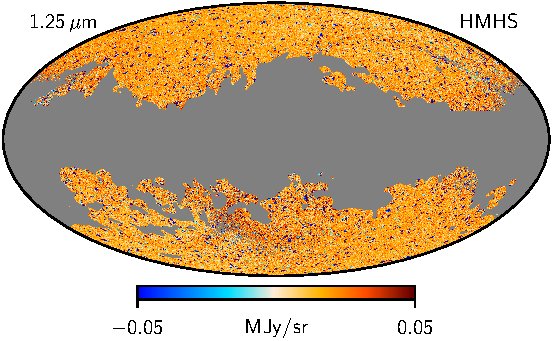
\includegraphics[width=0.40\linewidth]{figs/dirbe_01_hmhs_v1.pdf}\hspace*{5mm}
  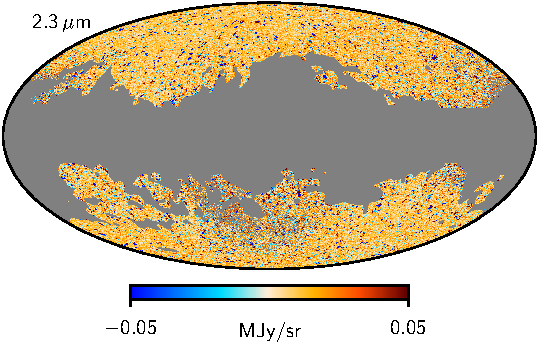
\includegraphics[width=0.40\linewidth]{figs/dirbe_02_hmhs_v1.pdf}\\
  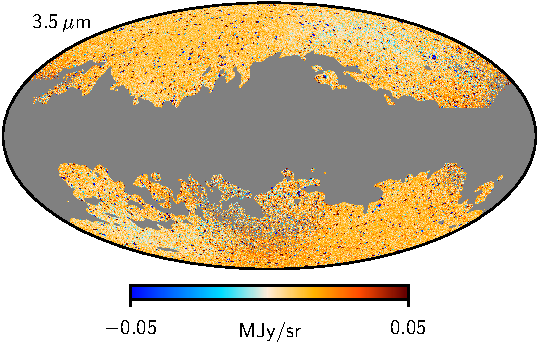
\includegraphics[width=0.40\linewidth]{figs/dirbe_03_hmhs_v1.pdf}\hspace*{5mm}
  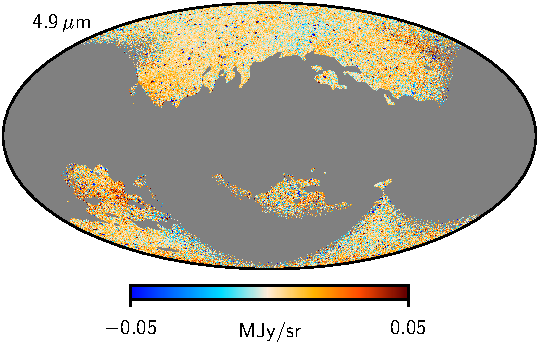
\includegraphics[width=0.40\linewidth]{figs/dirbe_04_hmhs_v1.pdf}\\
  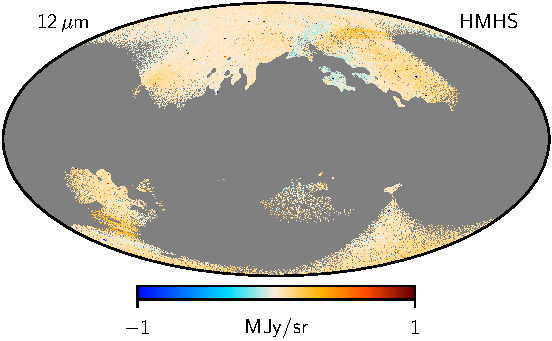
\includegraphics[width=0.40\linewidth]{figs/dirbe_05_hmhs_v1.pdf}\hspace*{5mm}
  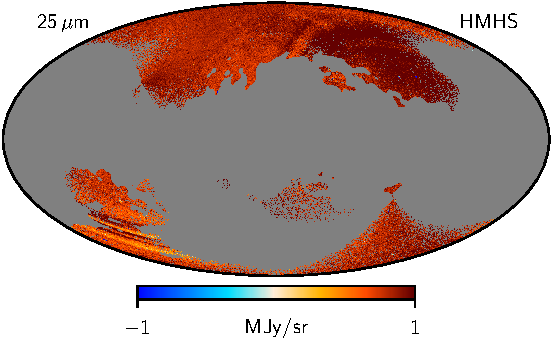
\includegraphics[width=0.40\linewidth]{figs/dirbe_06_hmhs_v1.pdf}\\
  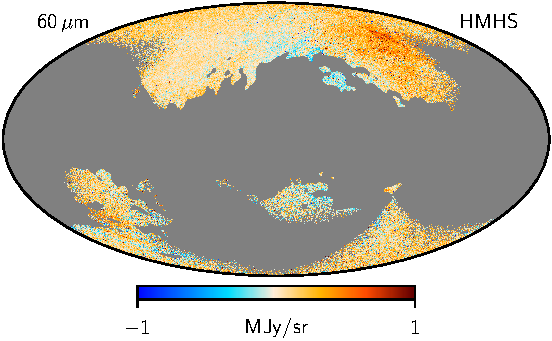
\includegraphics[width=0.40\linewidth]{figs/dirbe_07_hmhs_v1.pdf}\hspace*{5mm}
  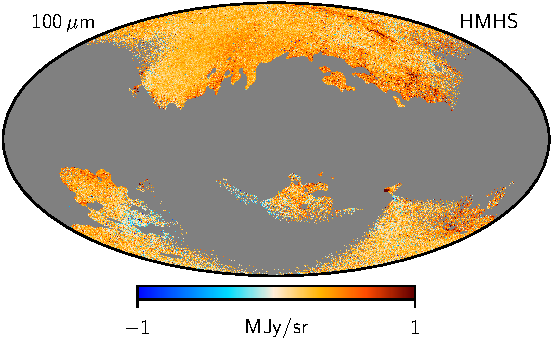
\includegraphics[width=0.40\linewidth]{figs/dirbe_08_hmhs_v1.pdf}\\
  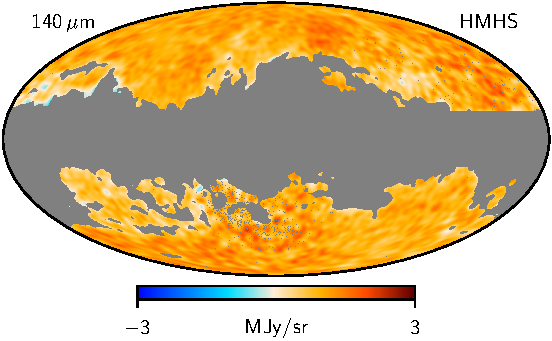
\includegraphics[width=0.40\linewidth]{figs/dirbe_09_hmhs_v1_3deg.pdf}\hspace*{5mm}
  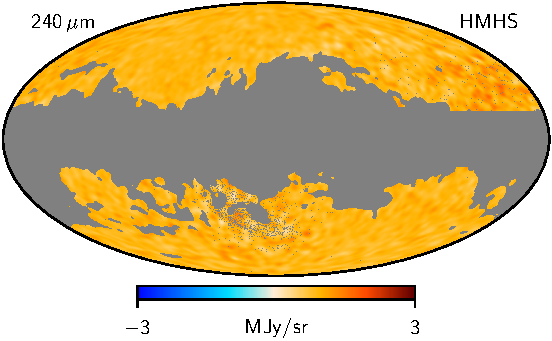
\includegraphics[width=0.40\linewidth]{figs/dirbe_10_hmhs_v1_3deg.pdf}
  \caption{Half-mission half-sum maps, $(\m_{\mathrm{HM1}}+\m_{\mathrm{HM2}})/2$ for each DIRBE frequency channel. Grey pixels indicate the union of a Galactic mask and the requirement that any pixels must be observed during both HM1 and HM2. }
  \label{fig:hmhs}
\end{figure*}

\begin{figure*}
  \centering
  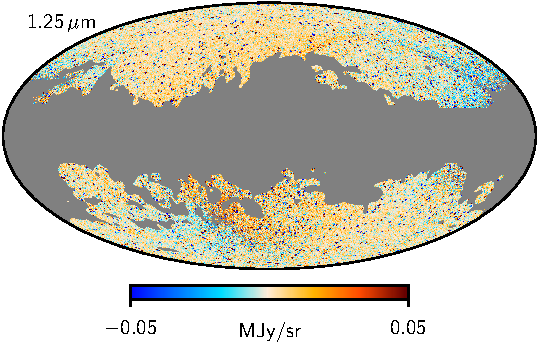
\includegraphics[width=0.40\linewidth]{figs/dirbe_01_hmhd_v1.pdf}\hspace*{5mm}
  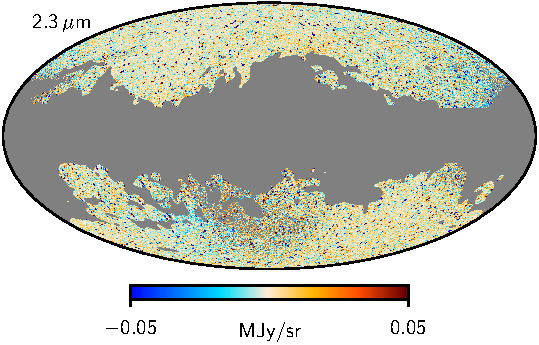
\includegraphics[width=0.40\linewidth]{figs/dirbe_02_hmhd_v1.pdf}\\
  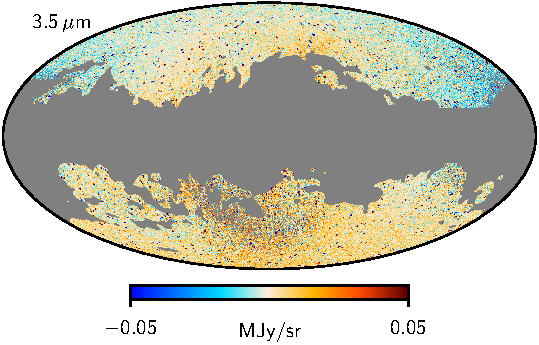
\includegraphics[width=0.40\linewidth]{figs/dirbe_03_hmhd_v1.pdf}\hspace*{5mm}
  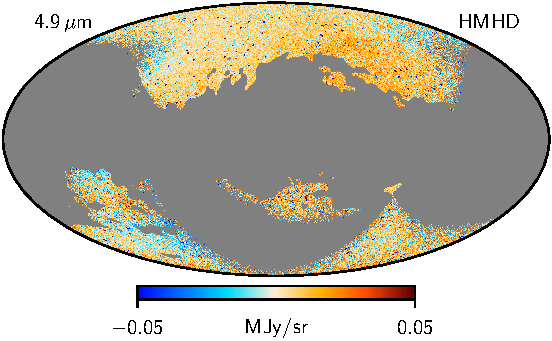
\includegraphics[width=0.40\linewidth]{figs/dirbe_04_hmhd_v1.pdf}\\
  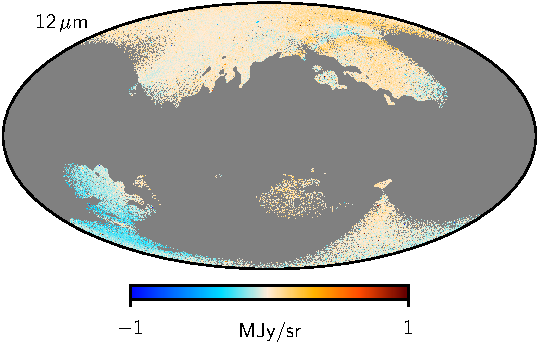
\includegraphics[width=0.40\linewidth]{figs/dirbe_05_hmhd_v1.pdf}\hspace*{5mm}
  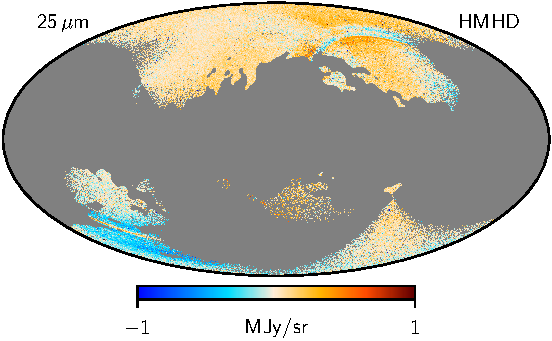
\includegraphics[width=0.40\linewidth]{figs/dirbe_06_hmhd_v1.pdf}\\
  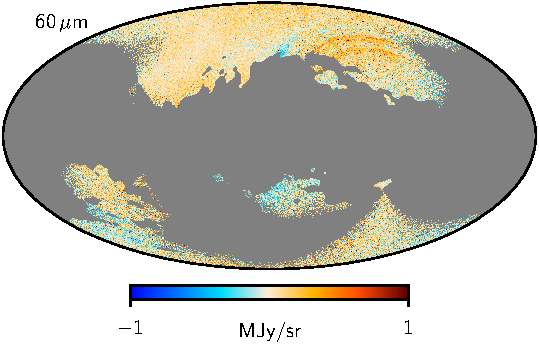
\includegraphics[width=0.40\linewidth]{figs/dirbe_07_hmhd_v1.pdf}\hspace*{5mm}
  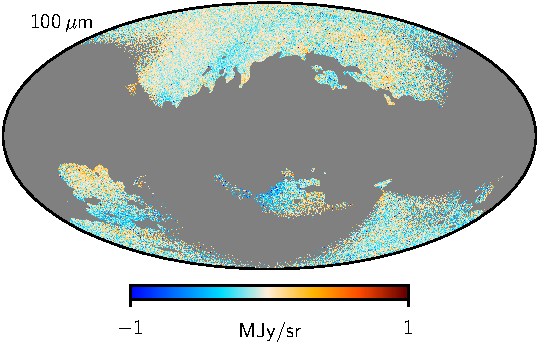
\includegraphics[width=0.40\linewidth]{figs/dirbe_08_hmhd_v1.pdf}\\
  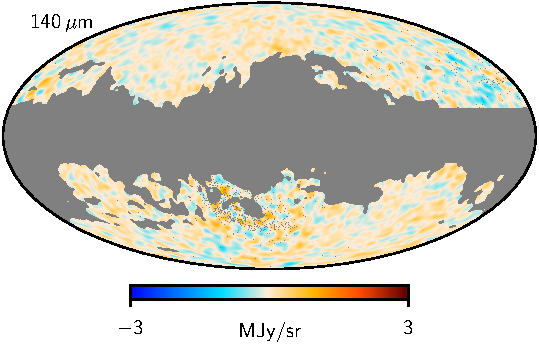
\includegraphics[width=0.40\linewidth]{figs/dirbe_09_hmhd_v1_3deg.pdf}\hspace*{5mm}
  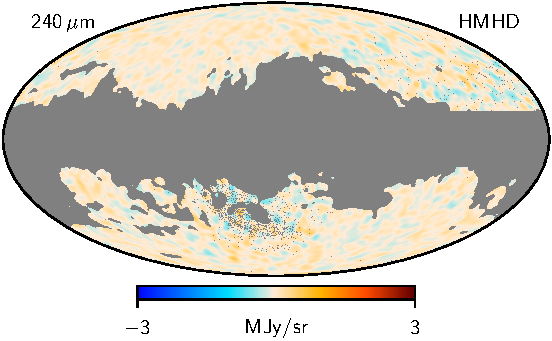
\includegraphics[width=0.40\linewidth]{figs/dirbe_10_hmhd_v1_3deg.pdf}
  \caption{Half-mission half-difference maps, $(\m_{\mathrm{HM1}}-\m_{\mathrm{HM2}})/2$ for each DIRBE frequency channel. Grey pixels indicate the union of a Galactic mask and the requirement that any pixels must be observed during both HM1 and HM2. }
  \label{fig:hmhd}
\end{figure*}

\begin{figure*}
  \centering
  %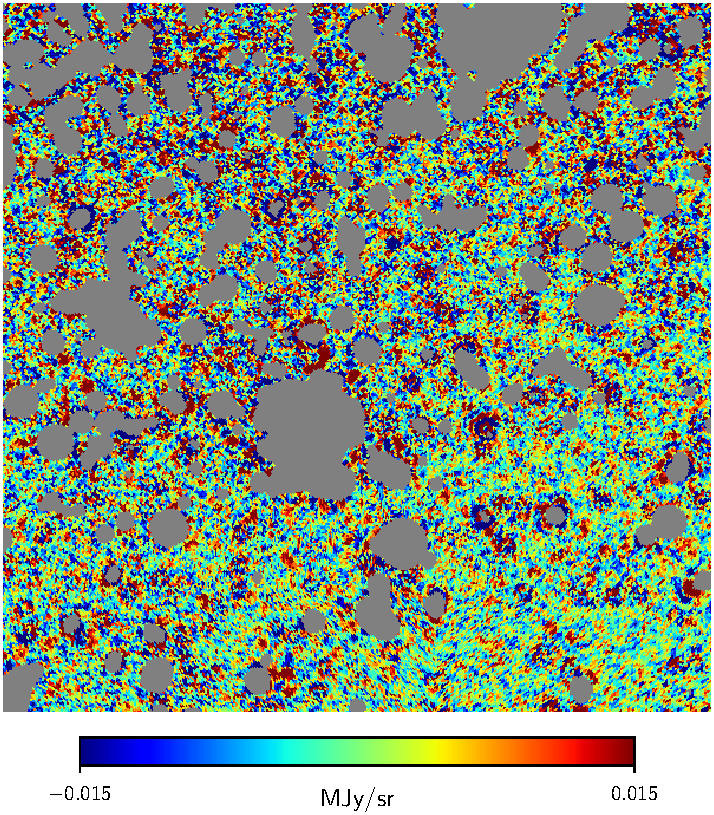
\includegraphics[width=0.23\linewidth]{figs/dirbe_01_hmhs_v1_zoom.pdf}\hspace*{5mm}
  %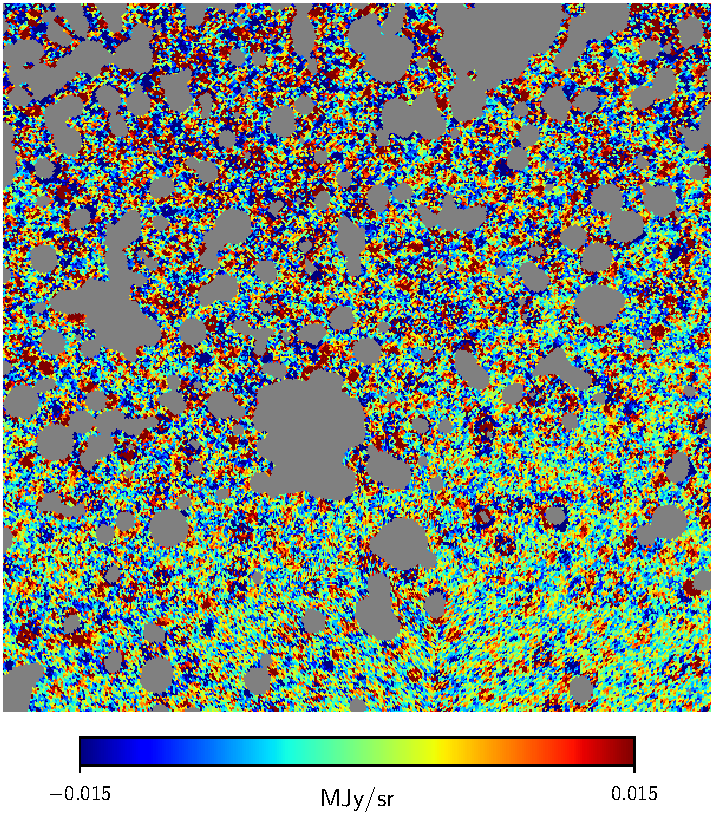
\includegraphics[width=0.23\linewidth]{figs/dirbe_02_hmhs_v1_zoom.pdf}\\
  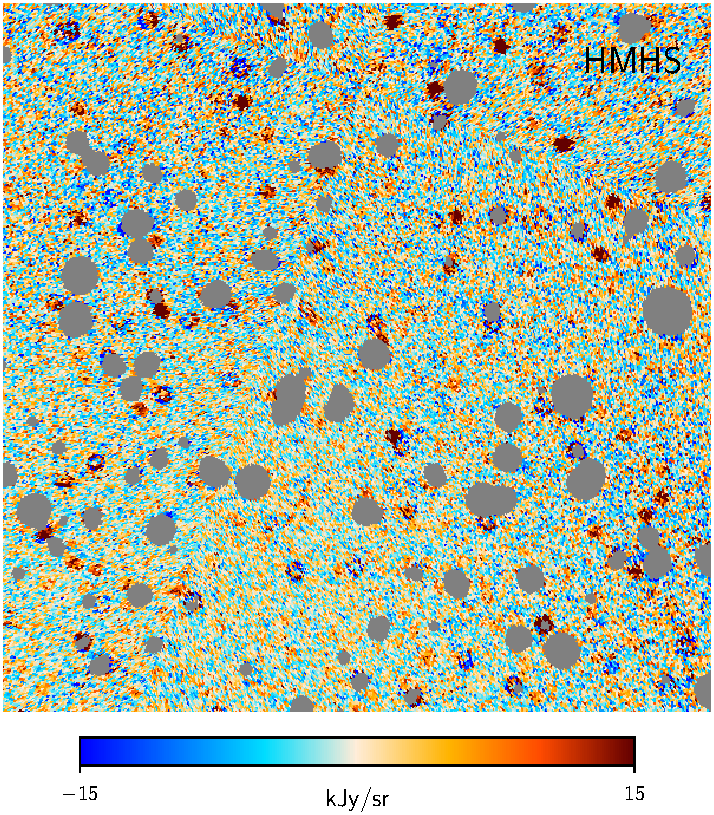
\includegraphics[width=0.45\linewidth]{figs/dirbe_03_hmhs_v1_zoom.pdf}\hspace*{0mm}
  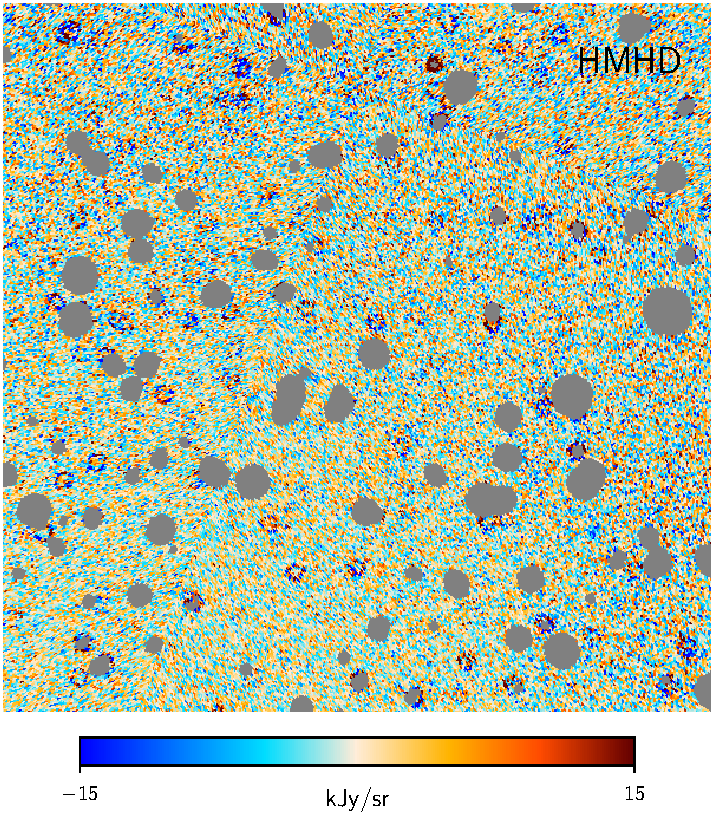
\includegraphics[width=0.45\linewidth]{figs/dirbe_03_hmhd_v1_zoom.pdf}
  %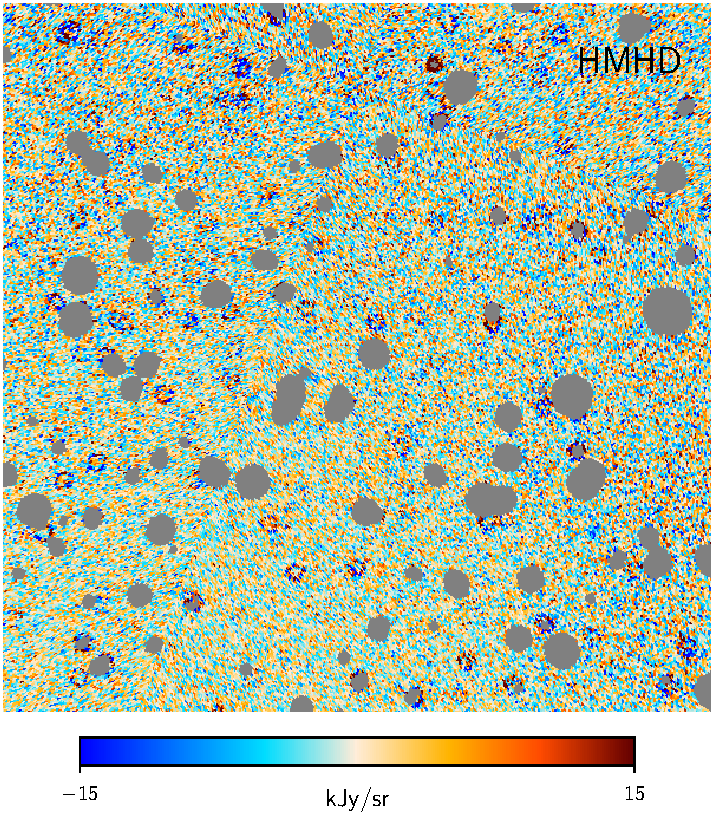
\includegraphics[width=0.45\linewidth]{figs/dirbe_03_hmhd_v1_zoom.pdf}\hspace*{5mm}
  %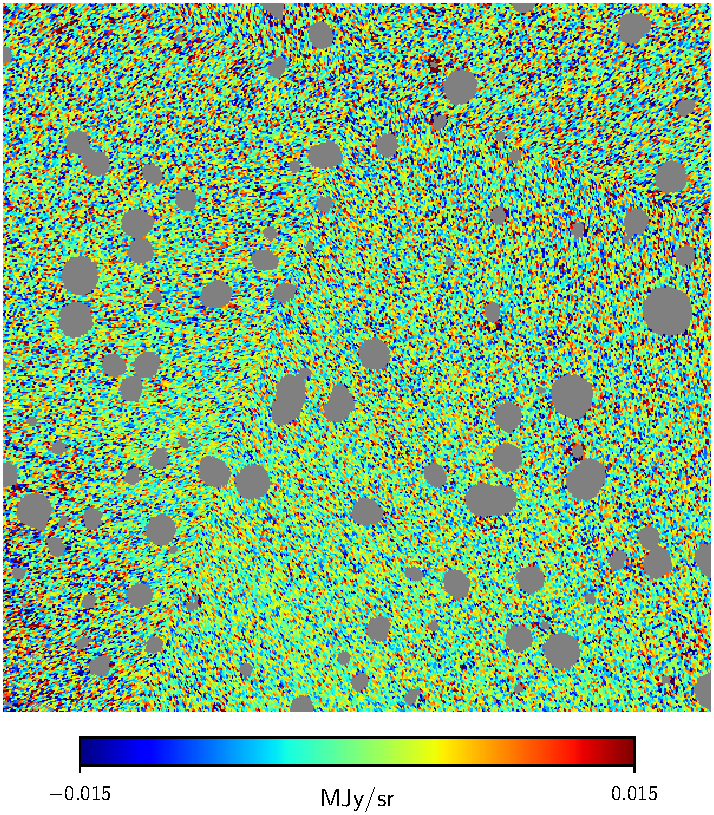
\includegraphics[width=0.45\linewidth]{figs/dirbe_04_hmhd_v1_zoom.pdf}
  %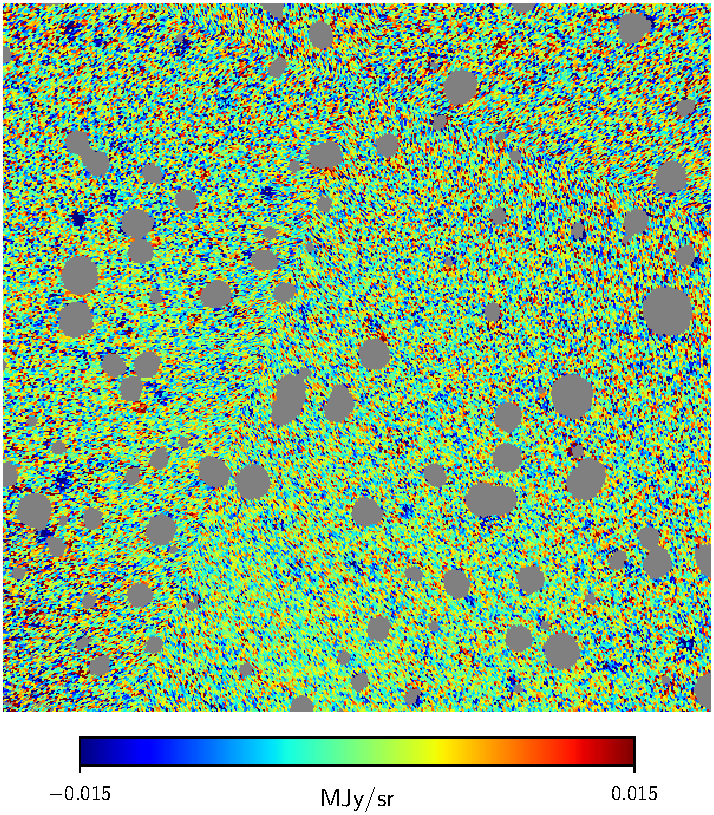
\includegraphics[width=0.23\linewidth]{figs/dirbe_04_hmhs_v1_zoom.pdf}\hspace*{5mm}
  %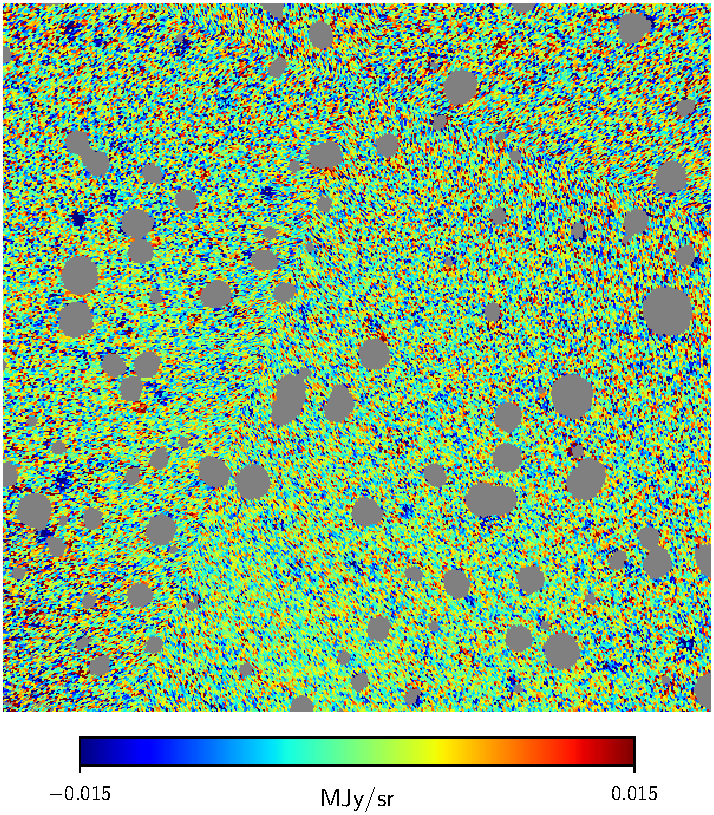
\includegraphics[width=0.23\linewidth]{figs/dirbe_04_hmhs_v1_zoom.pdf}\\
  %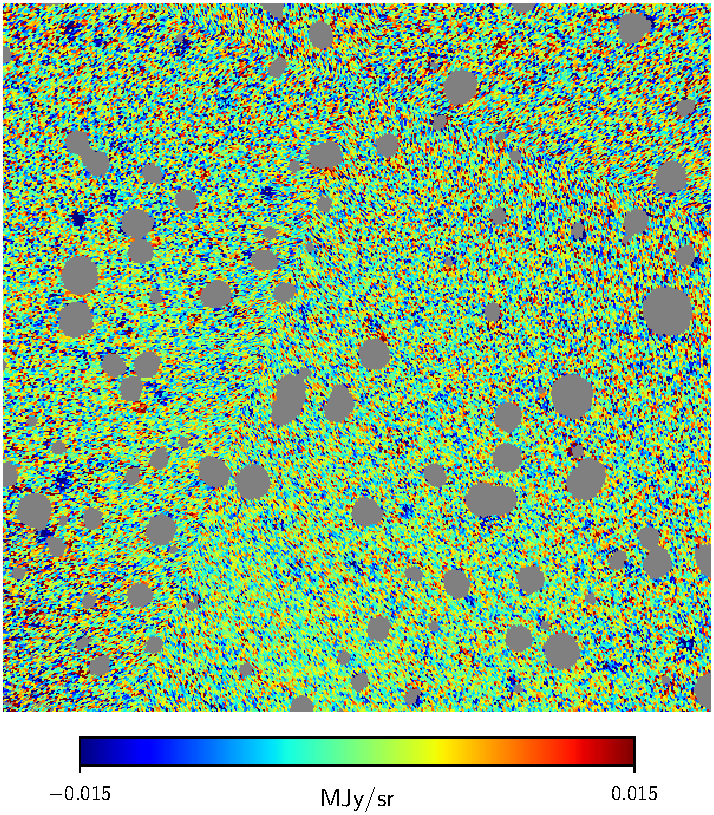
\includegraphics[width=0.23\linewidth]{figs/dirbe_04_hmhs_v1_zoom.pdf}\hspace*{5mm}
  %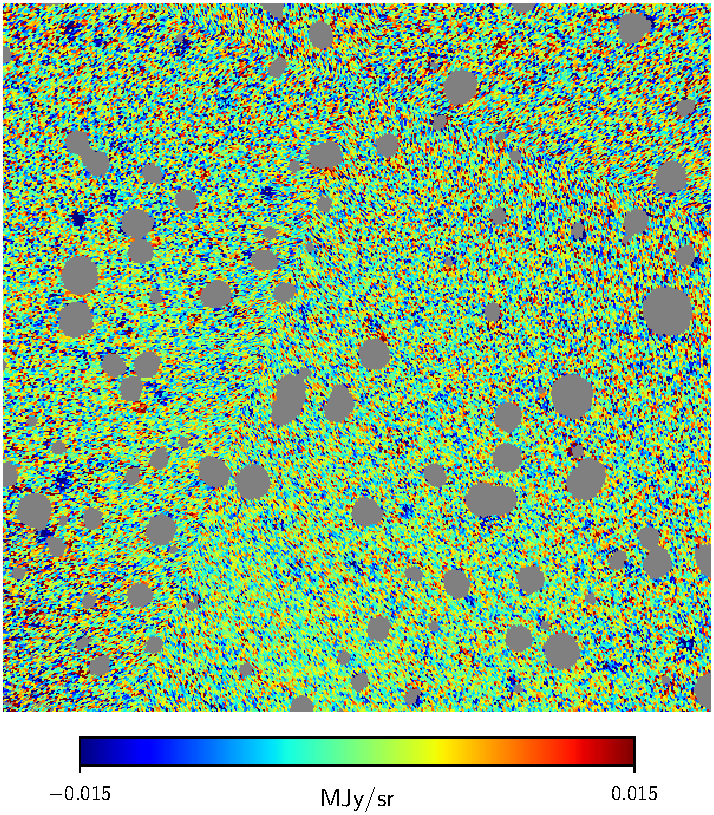
\includegraphics[width=0.23\linewidth]{figs/dirbe_04_hmhs_v1_zoom.pdf}\\
  %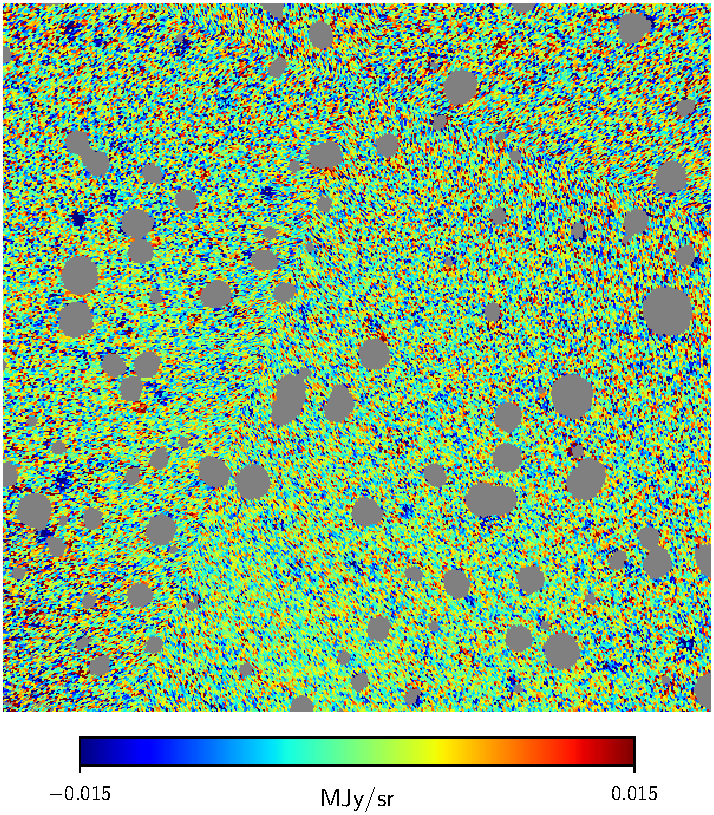
\includegraphics[width=0.23\linewidth]{figs/dirbe_04_hmhs_v1_zoom.pdf}\hspace*{5mm}
  %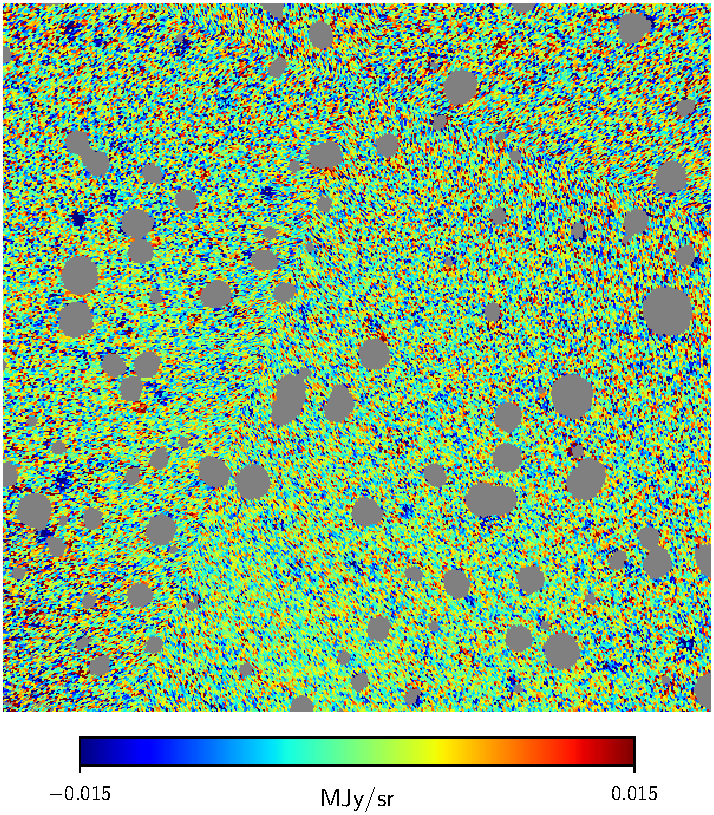
\includegraphics[width=0.23\linewidth]{figs/dirbe_04_hmhs_v1_zoom.pdf}
  \caption{Zoom-ins centered on Galactic coordinates $(l,b)=(90^{\circ},80^{\circ})$ of the half-mission half-sum maps, $(\m_{\mathrm{HM1}}+\m_{\mathrm{HM2}})/2$ for each DIRBE frequency channel. }
  \label{fig:hmhs_zoom}
\end{figure*}

%\begin{figure*}
%  \centering
%  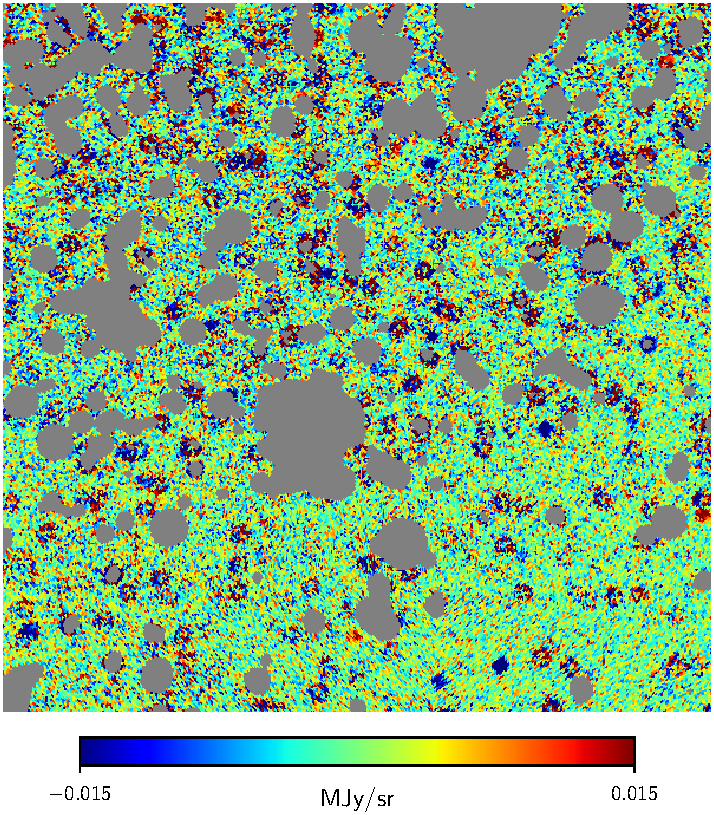
\includegraphics[width=0.23\linewidth]{figs/dirbe_01_hmhd_v1_zoom.pdf}\hspace*{5mm}
%  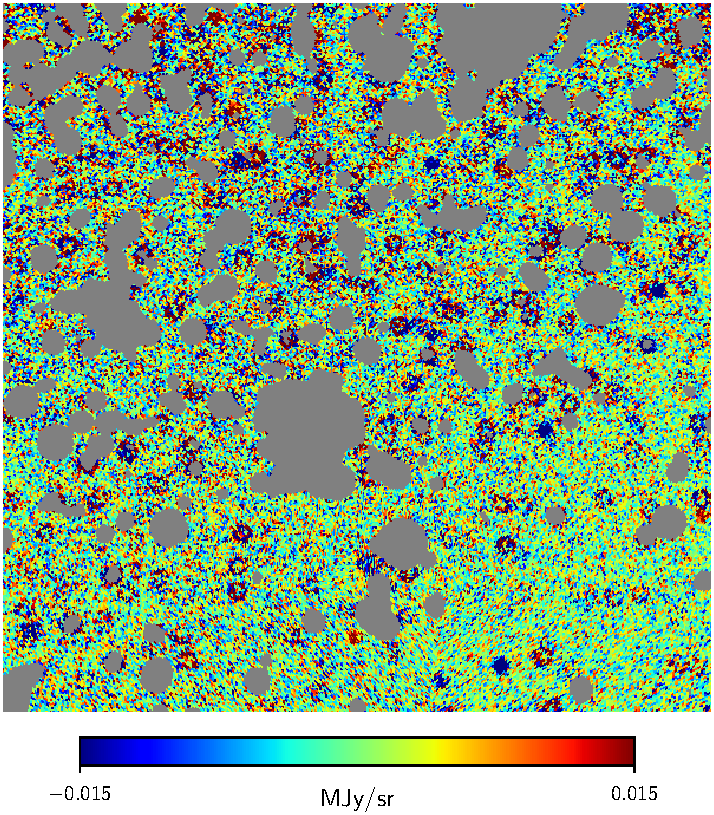
\includegraphics[width=0.23\linewidth]{figs/dirbe_02_hmhd_v1_zoom.pdf}\\
%  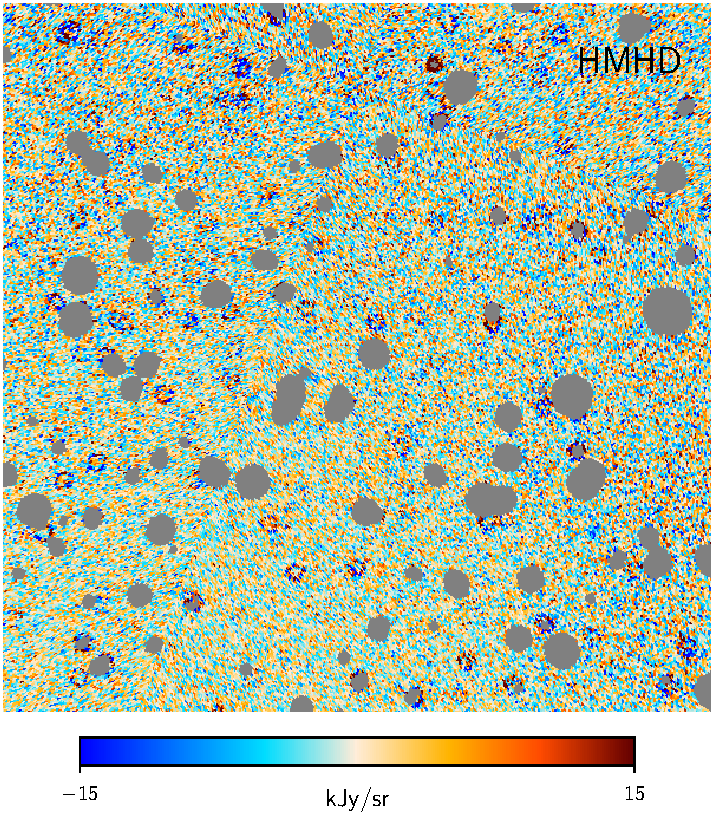
\includegraphics[width=0.23\linewidth]{figs/dirbe_03_hmhd_v1_zoom.pdf}\hspace*{5mm}
%  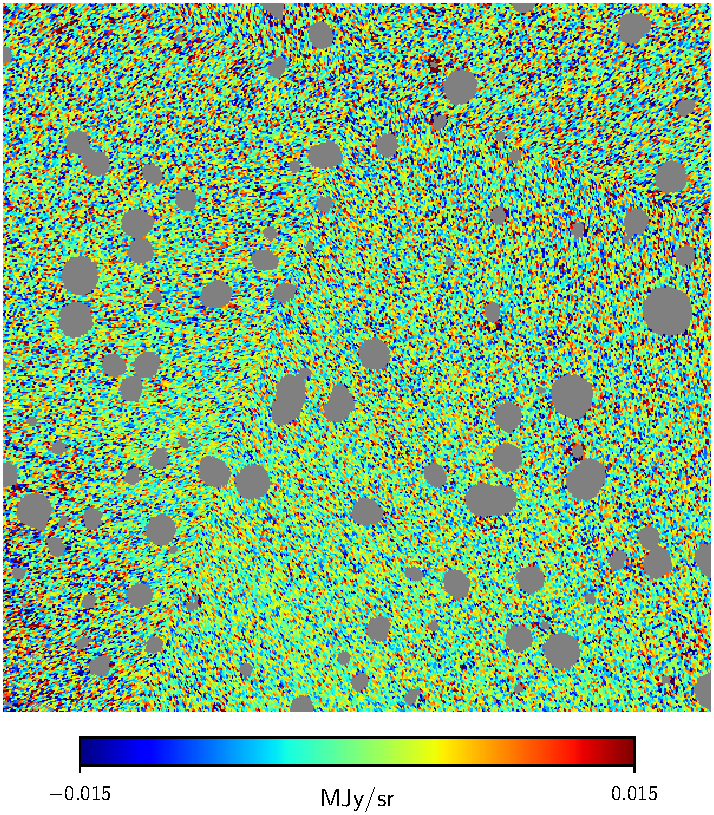
\includegraphics[width=0.23\linewidth]{figs/dirbe_04_hmhd_v1_zoom.pdf}\\
%  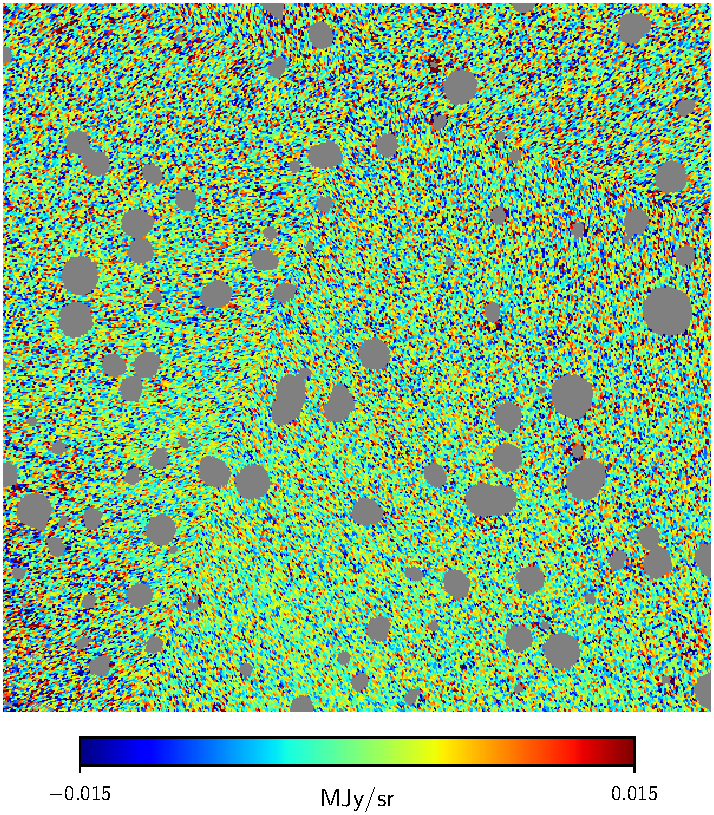
\includegraphics[width=0.23\linewidth]{figs/dirbe_04_hmhd_v1_zoom.pdf}\hspace*{5mm}
%  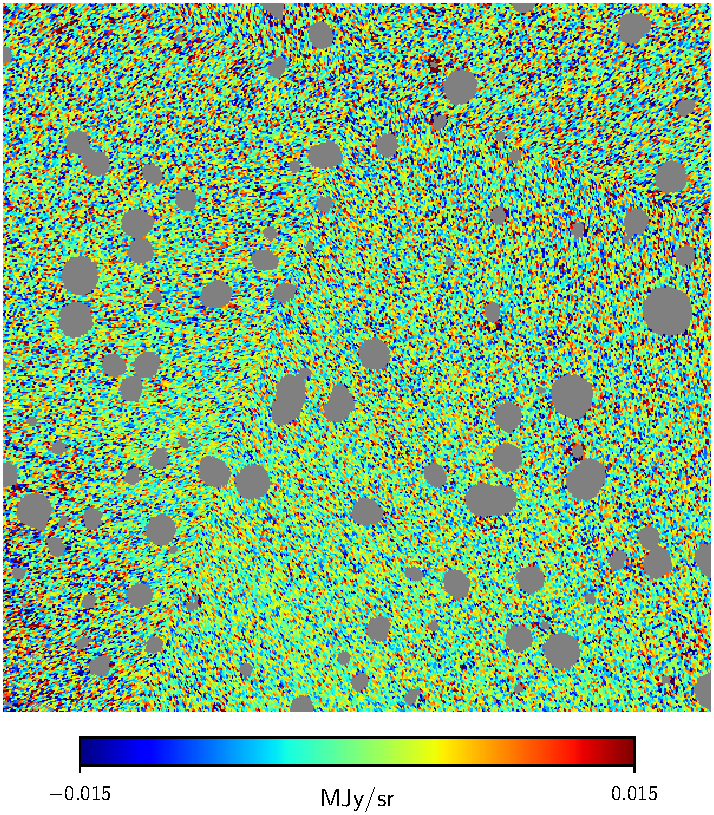
\includegraphics[width=0.23\linewidth]{figs/dirbe_04_hmhd_v1_zoom.pdf}\\
%  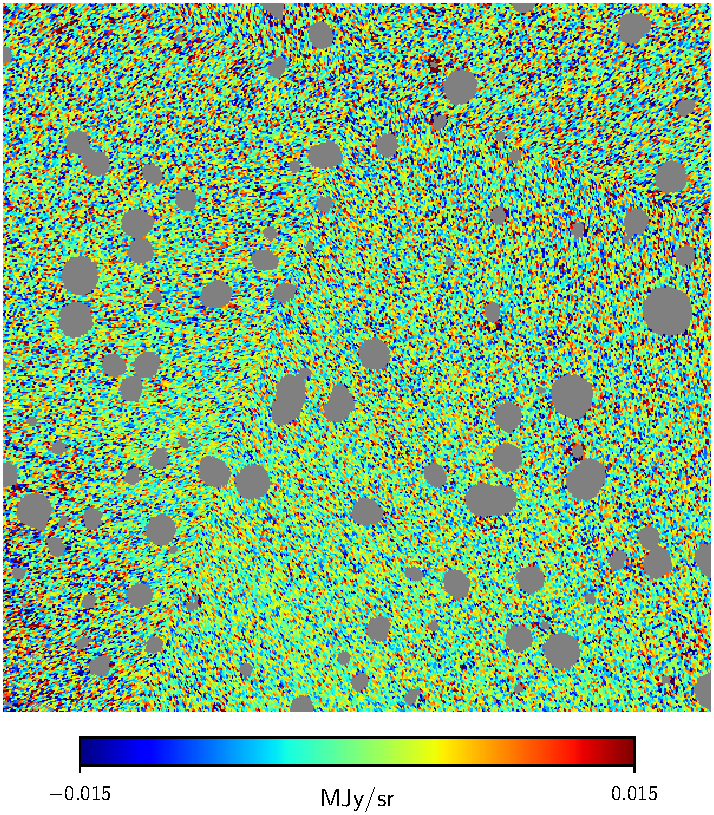
\includegraphics[width=0.23\linewidth]{figs/dirbe_04_hmhd_v1_zoom.pdf}\hspace*{5mm}
%  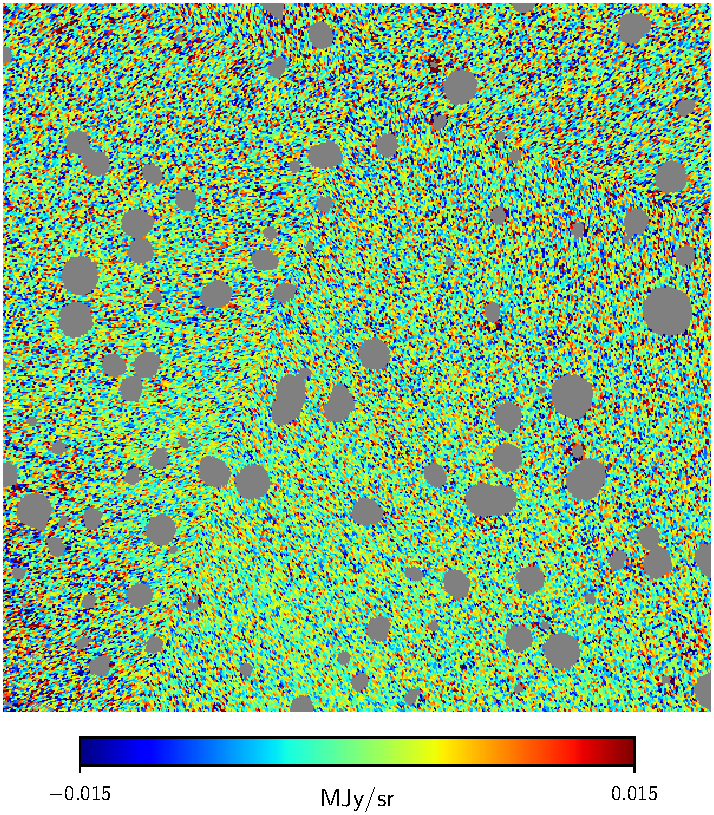
\includegraphics[width=0.23\linewidth]{figs/dirbe_04_hmhd_v1_zoom.pdf}\\
%  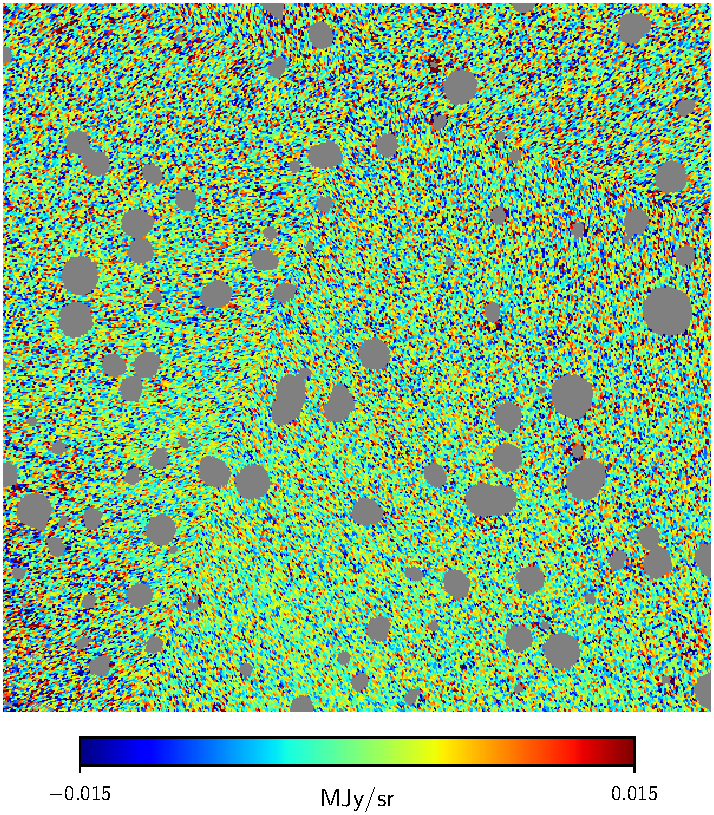
\includegraphics[width=0.23\linewidth]{figs/dirbe_04_hmhd_v1_zoom.pdf}\hspace*{5mm}
%  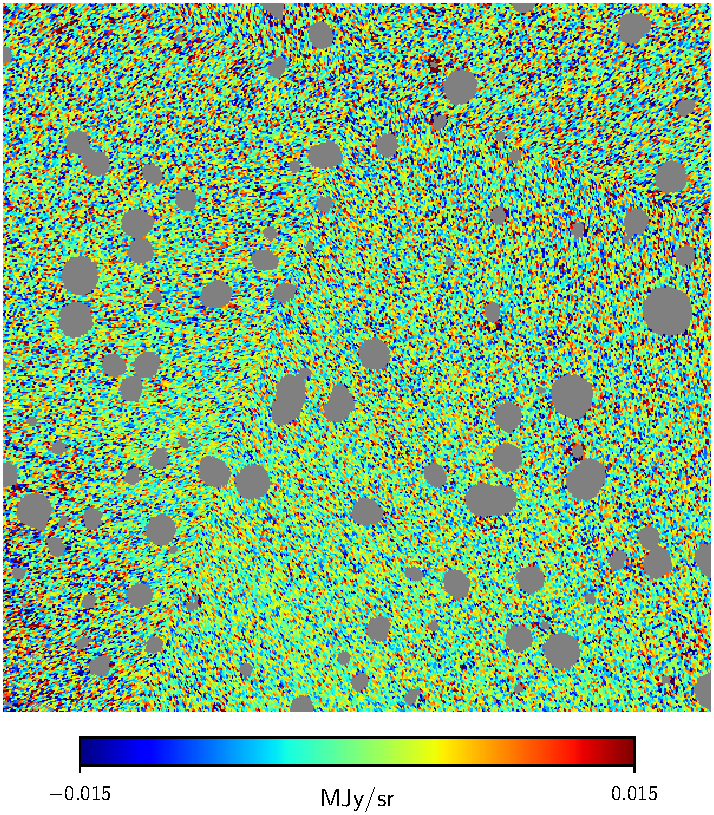
\includegraphics[width=0.23\linewidth]{figs/dirbe_04_hmhd_v1_zoom.pdf}
%  \caption{Zoom-ins centered on Galactic coordinates $(l,b)=(90^{\circ},80^{\circ})$ of the half-mission half-sum maps, $(\m_{\mathrm{HM1}}+\m_{\mathrm{HM2}})/2$ for each DIRBE frequency channel. }
%  \label{fig:hmhd_zoom}
%\end{figure*}

%\begin{figure}
%	\centering
%	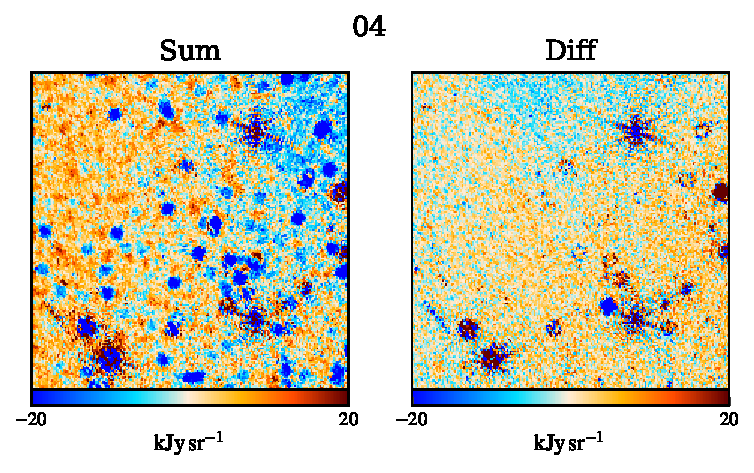
\includegraphics[width=\columnwidth]{figs/patch_04.pdf}
%	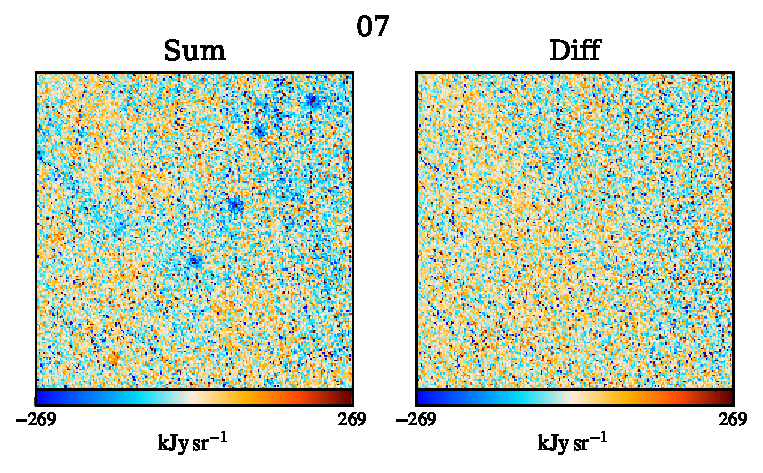
\includegraphics[width=\columnwidth]{figs/patch_07.pdf}
%	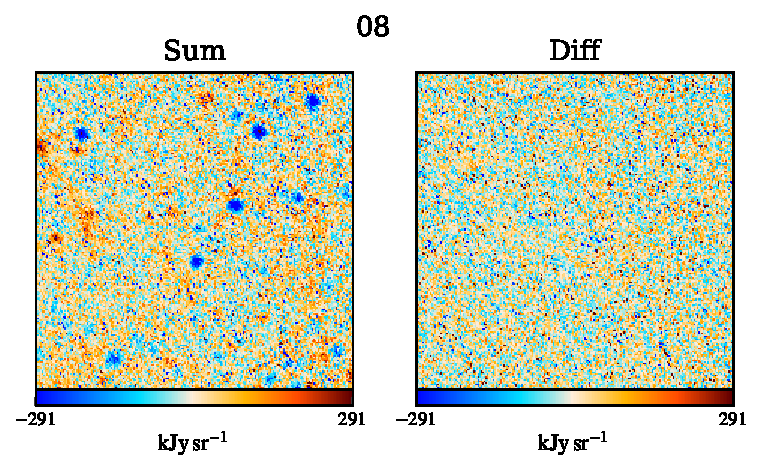
\includegraphics[width=\columnwidth]{figs/patch_08.pdf}
%	\caption{Half-sum and half-difference maps centered at $(l,b)=(67^\circ,56^\circ)$.}
%\end{figure}

\section{Monopoles}


Monopole values, comparison with zodi values, compared with theoretical predictions, previous limits, and previous detections.

\section{Power spectra}

Power spectra, comparison with GNILC, compare with theoretical predictions, previous limits, and previous detections.



\begin{figure*}
	\centering
	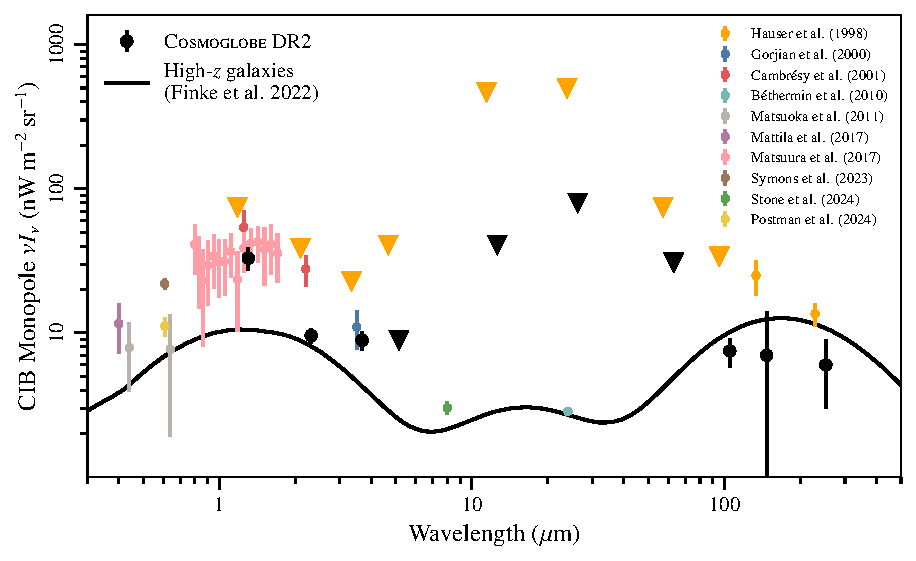
\includegraphics[width=0.8\textwidth]{figs/CIB_mono.pdf}
	\caption{Monopoles as measured by DIRBE, compared with theoretical predictions for EBL. Empty circles are DIRBE ZSMA maps with \textsc{Cosmoglobe} sky model removed.}
	\label{fig: EBL_monopoles}
\end{figure*}

\begin{figure*}
	\centering
	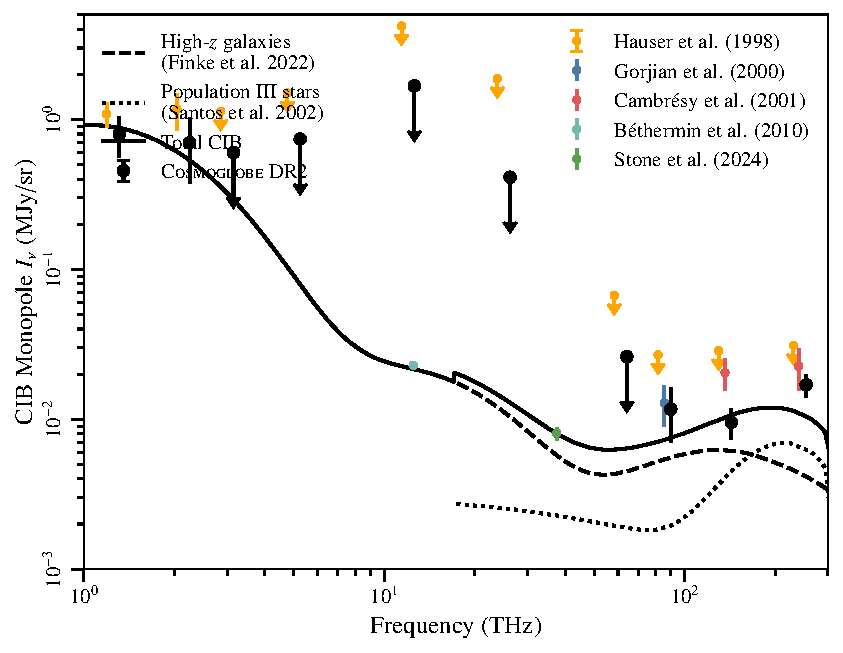
\includegraphics[width=0.8\textwidth]{figs/CIB_THz.pdf}
	\caption{Same as Figure \ref{fig: EBL_monopoles}, but with different units.}
	\label{fig: EBL_monopoles_THz}
\end{figure*}

\section{Conclusions}

This is the first time that CIB fluctuations have been detected in DIRBE, and the first time that fluctuations and monopoles have been detected in the same band.

As demonstrated here, the limitation in fully modeling the CIB has been the inability to properly utilize external data. In this work, the reanalysis of DIRBE data was made much simpler not only by the large increase of relative computing power with respect to dataset size, but also the information gained by using a global sky model spanning from $100\,\mathrm{GHz}$ to $1\,\mathrm{\mu m}$.

Much of this work is made possible through the use of archival time-ordered data with complementary scan strategies, frequency coverage, detector technologies, and observation time. In the case of CIB studies, the interplay between foregrounds, namely zodiacal and Galactic dust, has limited previous detections. In future work, additional data will further break these degeneracies, and the potential to further understand the astrophysical signals in these datasets will be improved. In particular, the \textit{Infrared Astrophysical Observatory} (\textit{IRAS}) created nearly full-sky maps at 12, 25, 60, and 100 $\mathrm{\mu m}$ with resolution between 0.5 arcmin to 2 arcmin. A full end-to-end joint analysis of \textit{IRAS} and DIRBE will leverage the unique properties of both datsets, and enable an even deeper view of the CIB in the tens of microns.

\begin{acknowledgements}
 The current work has received funding from the European
  Union’s Horizon 2020 research and innovation programme under grant
  agreement numbers 819478 (ERC; \textsc{Cosmoglobe}) and 772253 (ERC;
	\textsc{bits2cosmology}). Some of the results in this paper have been derived using healpy \citep{Zonca2019} and the HEALPix \citep{healpix} package.
  We acknowledge the use of the Legacy Archive for Microwave Background Data
  Analysis (LAMBDA), part of the High Energy Astrophysics Science Archive Center
  (HEASARC). HEASARC/LAMBDA is a service of the Astrophysics Science Division at
  the NASA Goddard Space Flight Center.  
\end{acknowledgements}


%-------------------------------------------------------------
%                                       Table with references 
%-------------------------------------------------------------
%

\bibliographystyle{aa}
\bibliography{../../common/Planck_bib,../../common/CG_bibliography}

\end{document}
%%%% End of aa.dem
